%!TEX root = ../../main.tex
\chapter{調性制約の生成}
本章では調性制約の生成方法について述べる
%--------%---------%---------%--------%---------%---------
\section{調性制約の形式}
調性制約は,曲のコード進行に応じて出力可能な音の周波数列を変化させている.本研究では調性制約は時間(ms),出力可能な周波数列のcsvファイルとして生成され,周波数列の選び方は(1)コードの構成音のみ.(2)コードの構成音+コードに対するメロディ頻度の高い音.の2種類の調性制約を生成した.
\subsection{コードに対するメロディ頻度のカウント}
Songleからのコードとメロディのデータ100曲分を使用してその統計をとる.まず,コードを表\ref{tab:convert}に従って別のコードに分類する.表\ref{tab:convert}は100曲分のコードで出現頻度の高いコードのみを載せている.分類後の各コードのときCからBまでの1オクターブ分12音が流れている時間を計測し,調の主音からの相対的な位置が等しいコードとメロディをまとめてカウントする.例えば,調の主音AのときのコードAでメロディG\#が流れた場合と,調の主音CのときのコードCでメロディBが流れた時は同じ物としてカウントする.こうしてカウントしたメロディのながさの合計(ms)を各コードのメロディ出現頻度とした.メロディの周波数が1オクターブの範囲を超える場合は,オクターブ般化を行ってからカウントする.カウントは長調と短調は分けてカウントした.図\ref{img:MIM},図\ref{img:MIVM},図\ref{img:MVM}にそれぞれ長調のときのコードIM,コードIVM,コードVMのときの各メロディの出現頻度を,図\ref{img:mIM}PFG Tonnetz上に表示したものをそれぞれ示す.
図\ref{img:MIM},図2\ref{img:MIVM},図3\ref{img:MVM}を比べると
コードの根音が5度上にあがるとグラフの平面上でコードの三和音が右に平行移動したが,
5度さがったとき単純な平行移動ではなく根音ではなく主音の頻度のほうが大きい.
構成音以外の音の違いは
根音の左上(6度)右上(7度)を比べると図\ref{img:MIM}、図\ref{img:MIVM}は同じくらいで図\ref{img:MVM}は右上がかなりすくない.
図\ref{img:MIM}と図\ref{img:mIM}を比べると同じコードでもメロディ頻度の分布に違いが生じていて,短調のほうは原点の下側の領域に分布が出やすくなっている.
\subsection{周波数列の決定}
調性制約がもつ(2)の周波数列を決定する時に,コードに対するメロディの出現頻度から決める.コードの構成音に加えて,構成音以外でメロディ頻度が一番高いものを基準にその音に経験的に設定した倍率をかけた値と,コードに対するメロディの割合を閾値としてその閾値を上回った音を周波数列に加える.経験的に設定した倍率や閾値はコード構成音以外の音の頻度を降順にソートして平均をとって設定した.
 \begin{table}[t]
     \caption{コード変換表}
     \begin{center}
         \begin{tabular}{ | c | c || c | c | } \hline
         	変換前 & 変換後 & 変換前 & 変換後 \\ \hline \hline
			XM & XM &Xsus4 & XM \\ \hline
			X-13 & XM & Xadd2 & XM \\ \hline
			X-11 & XM & Xadd4 & XM \\ \hline
			X-9 & XM & Xadd9 & XM \\ \hline
			X-9 & X7 & Xaug & XM \\ \hline
			X-5 & XM & XaugM7 & XM7 \\ \hline
			X-4 & X7 & Xdim & Xm \\ \hline
			X6 & X6 & Xdim7 & Xm \\ \hline
			X7 & X7 & Xm & Xm \\ \hline
			X9 & X7 & Xm11 & Xm7 \\ \hline
			X11 & X7 & Xm13 & Xm7 \\ \hline
			X13 & X7 & Xm6 & Xm \\ \hline
			X7-5 & X7 & Xm7 & Xm7 \\ \hline
			X7-9 & X7 & XM7 & XM7 \\ \hline
			X7-Aug & X7 & Xm7-9 & Xm7\\ \hline
			X9-Aug & X7 & Xm9 & Xm7 \\ \hline
			X9-5 & X7 & XM9 & XM7 \\ \hline
			X7+11 & X7 & Xmadd9 & Xm7 \\ \hline
			X7+13 & X7 & XmM7 & Xm \\ \hline
			X7+9 & X7 & Xsus2 & XM \\ \hline
			X7b5 & X7& Xsus4 & XM \\ \hline
         \end{tabular}
         \label{tab:convert}
     \end{center}
 \end{table}
 
\begin{figure}[t]
	\begin{center}
		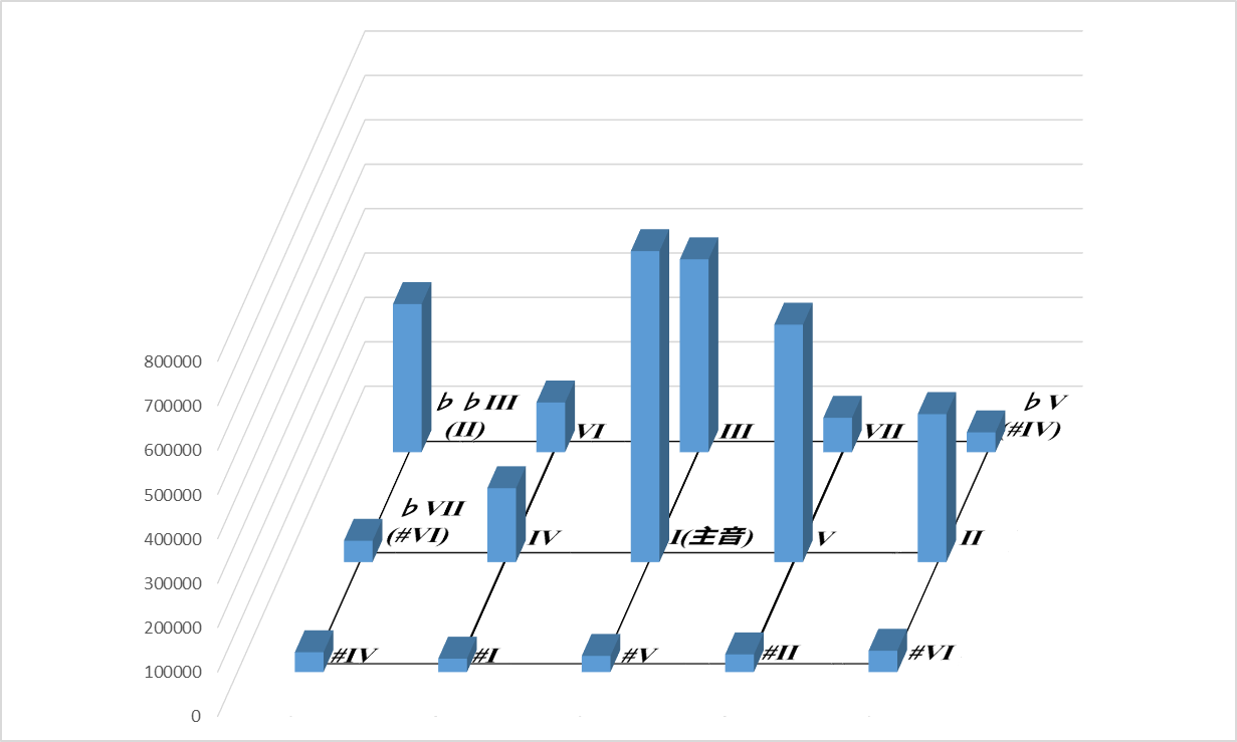
\includegraphics[width=0.8\linewidth]{./pics/05/MajorIM.png}
		\caption{長調のコードIMの各メロディの出現頻度}
		\label{img:MIM} 
	\end{center}
\end{figure}
\begin{figure}[t]
	\begin{center}
		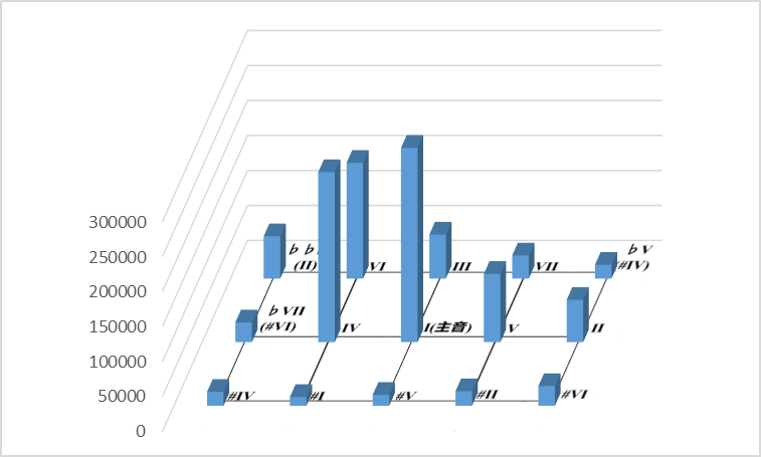
\includegraphics[width=0.8\linewidth]{./pics/05/MajorIVM.png}
		\caption{長調のコードIVMの各メロディの出現頻度}
		\label{img:MIVM} 
	\end{center}
\end{figure}
\begin{figure}[t]
	\begin{center}
		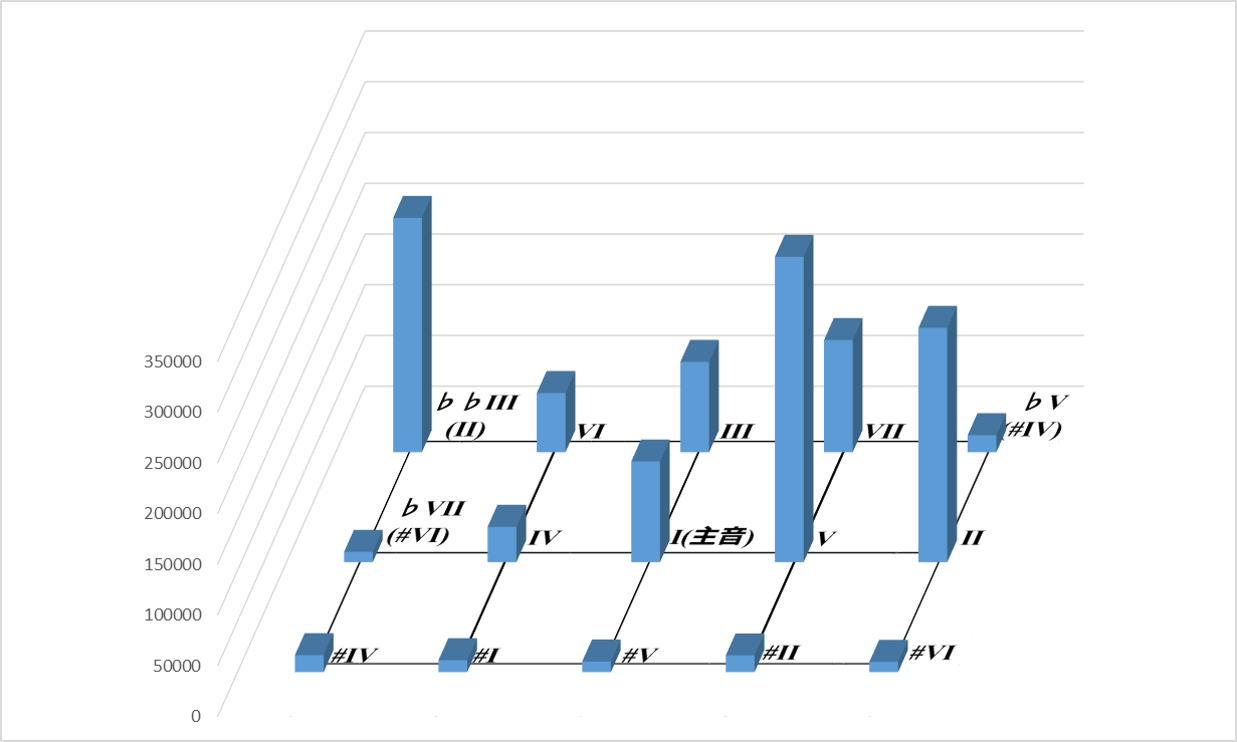
\includegraphics[width=0.8\linewidth]{./pics/05/MajorVM.png}
		\caption{長調のコードVMの各メロディの出現頻度}
		\label{img:MVM} 
	\end{center}
\end{figure}
\begin{figure}[t]
	\begin{center}
		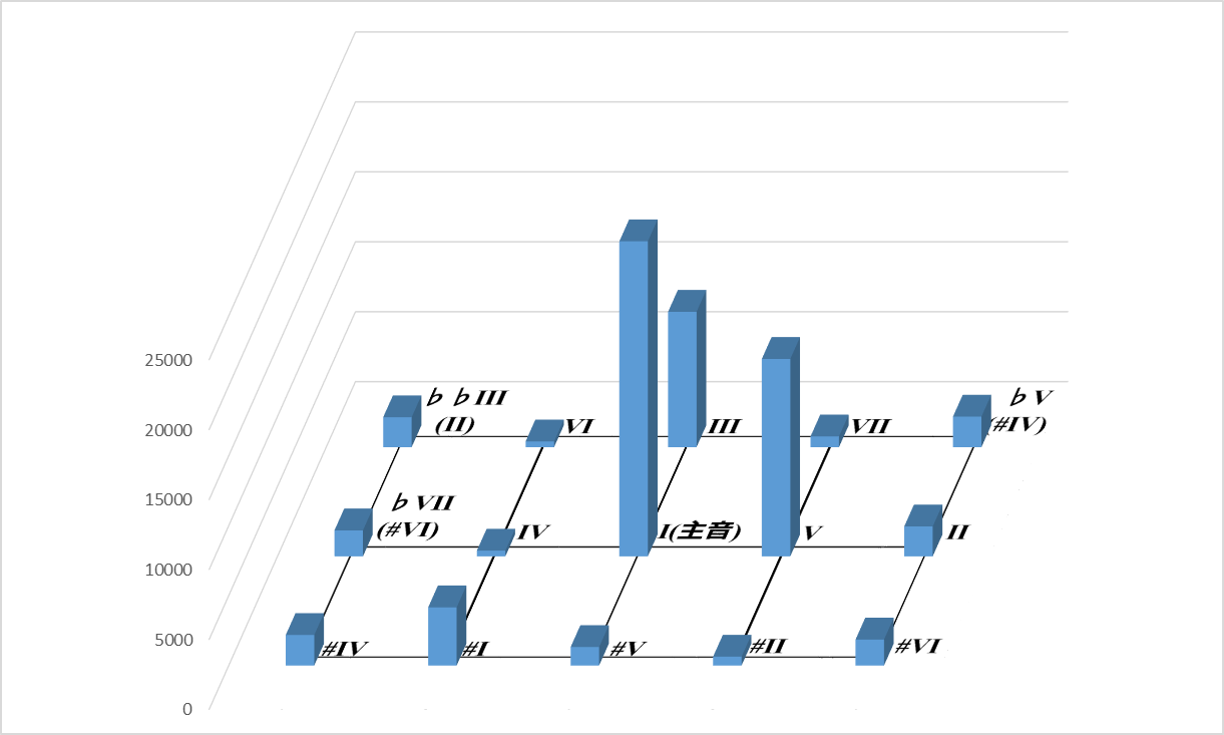
\includegraphics[width=0.8\linewidth]{./pics/05/minorIM.png}
		\caption{短調のコードIMの各メロディの出現頻度}
		\label{img:mIM} 
	\end{center}
\end{figure}